\documentclass[10pt]{article}

\usepackage[margin=1in]{geometry}
\usepackage{amsmath,amsfonts,amssymb,bm}
\usepackage{booktabs}
\usepackage{graphicx}
\usepackage{multirow}
\usepackage{array}
\usepackage{url}
\usepackage{xcolor}
\usepackage{caption}
\usepackage{subcaption}
\usepackage[numbers,sort&compress]{natbib}

\graphicspath{{../paper_assets/neurips_closure_2026-04-28/figures/}{../figures/}{../figures/paper/}}

\newcommand{\method}{\textsc{DOOR-RL}}
\newcommand{\ours}{\textsc{TypeBudget}}
\newcommand{\kctx}{K}
\newcommand{\kdyn}{K_{\mathrm{dyn}}}
\newcommand{\krel}{K_{\mathrm{rel}}}
\newcommand{\cdyn}{\mathcal{C}_{\mathrm{dyn}}}
\newcommand{\sdyn}{\mathcal{S}_{\mathrm{dyn}}}
\newcommand{\srel}{\mathcal{S}_{\mathrm{rel}}}
\newcommand{\miss}{\mathrm{MissRate}}
\newcommand{\cdr}{\mathrm{CDR}}
\newcommand{\wasted}{\mathrm{WastedRel}}
\newcommand{\todo}[1]{\textcolor{red}{[TODO: #1]}}

\title{\vspace{-1.0em}When Relations Compete with Objects: Budget-Aware Token Abstraction for Driving World Models}

\author{
Anonymous Authors\\
Paper draft for NeurIPS submission\\
\texttt{anonymous@example.com}
}

\date{}

\begin{document}
\maketitle

\begin{abstract}
Object-relational world models provide a structured interface for autonomous driving, but they must often operate under a limited latent context budget. We show that this setting creates a previously under-examined failure mode: \emph{type competition}. Object tokens are state-bearing entities, while relation tokens encode sparse but decision-dense cues such as time-to-collision and interaction risk. A unified top-$K$ selector treats these heterogeneous tokens as exchangeable, causing relation tokens to displace critical dynamic agents or become ungrounded when their endpoint objects are absent from the latent state. We propose a budget-aware, type-aware token abstraction that allocates separate capacity to dynamic agents and relation edges under the same total world-model context budget. To expose the mechanism, we introduce selection diagnostics including Critical Dynamic Retention and Relation Wasted Slot Rate. Across nuScenes and nuPlan, our abstraction improves limited-budget representation sufficiency, reduces critical-agent misses and wasted relation slots, and yields more stable latent planning performance. Our results suggest that relation-aware driving world models require not only richer relation tokens, but also budget-aware mechanisms that keep those relations grounded in retained dynamic state.
\end{abstract}

\section{Introduction}
Structured world models are an increasingly attractive substrate for autonomous driving. Rather than compressing a scene into a single global vector, object-relational representations expose the entities and interactions that matter for decision making: the ego vehicle, nearby vehicles, pedestrians and cyclists, lane-level context, and interaction cues such as time-to-collision, conflict, and priority. Such structure is especially useful for planning, where rare but safety-critical entities and their relations often dominate the correct action.

Yet object-relational structure creates a practical bottleneck. A real driving scene can contain many object, map, signal, and relation tokens, while the downstream world model and policy typically consume only a limited context. This forces a token abstraction problem: which subset of tokens should be retained in the latent state? A common answer is to score all tokens and keep a unified top-$K$ set. This design is simple, but it silently assumes that all token types are exchangeable under a shared budget.

We argue that this assumption is wrong for driving world models. Object tokens and relation tokens play different roles. Object tokens are \emph{state-bearing}: they carry the physical states that must be predicted forward. Relation tokens are \emph{decision-dense}: they may encode sparse but high-value signals such as low TTC, lane conflict, or interaction risk. Moreover, the value of a relation token depends on its endpoints. A selected relation whose associated dynamic agent is missing from the latent state is not a useful relational fact; it is an orphan relation. Under a fixed shared top-$K$ budget, relation tokens and object tokens therefore do not merely add information to each other. They compete.

This paper studies the resulting failure mode, which we call \emph{type competition}. In a limited-capacity object-relational world model, a unified selector can allocate slots to relation tokens while missing critical dynamic agents. The failure is subtle because the selected relations may appear semantically meaningful in isolation, yet the latent state lacks the entities needed to ground them. In prediction and planning, this manifests as poor dynamic-agent retention, degraded rare-agent forecasting, lower interaction recall, and unstable downstream latent policy learning.

We propose a simple but important alternative: budget-aware type abstraction. Instead of applying one top-$K$ selector to the union of objects and relations, we allocate separate budgets to dynamic-agent tokens and relation tokens while keeping the total world-model context budget fixed. In our implementation, a 16-slot context is split into a dynamic path and a relation path, with independent selectors and type-aware supervision. Dynamic slots predict physical next-state quantities, while relation slots predict decision-relevant edge semantics. The selector score itself remains learned and ego-conditioned; our change is not a hand-crafted rule for distance or TTC, but a structural constraint on how learned scores spend capacity across token types.

Our contributions are:
\begin{enumerate}
    \item We identify \emph{type competition} as a failure mode of limited-capacity object-relational world models for driving.
    \item We propose a decision-sufficient, budget-aware, type-aware token abstraction that separates dynamic-agent and relation selection under a fixed total context budget.
    \item We introduce selection diagnostics that quantify critical-agent misses and orphan relations, linking selector behavior to downstream interaction errors.
    \item We provide prediction-to-planning evidence across nuScenes and nuPlan, including representation sufficiency, latent planning, relation semantic ablations, and external-style imitation baselines.
\end{enumerate}

\section{Related Work}
\paragraph{World models for driving.}
World models support imagination-based policy learning by predicting future latent states under candidate actions \citep{ha2018worldmodels,hafner2023dreamerv3}. For autonomous driving, this is appealing because closed-loop data collection and policy search are expensive and safety-critical. Existing work in driving simulators and planning benchmarks further shows that evaluation regime matters: nuScenes emphasizes perception and prediction, while nuPlan, CARLA, Waymax, and NAVSIM expose different planning and simulation interfaces \citep{caesar2020nuscenes,caesar2021nuplan,dosovitskiy2017carla,mao2023waymax,dauner2024navsim}.

\paragraph{Object-centric and relational representations.}
Object-centric learning decomposes scenes into entity-like slots, improving compositionality and interpretability in structured domains \citep{locatello2020slotattention}. Autonomous driving naturally fits this view: the policy must track vehicles, vulnerable road users, lanes, and interaction cues. Our focus is not merely whether relation tokens are useful, but how object and relation tokens should share limited context in a downstream world model.

\paragraph{Decision-sufficient abstraction.}
For planning, a good representation need not reconstruct every scene detail. It should preserve the variables needed to predict decision-relevant futures and select actions. We operationalize this with both prediction metrics and selection diagnostics: a representation should retain critical dynamic agents and relation semantics that influence downstream planning, while avoiding ungrounded relation slots.

\section{Problem Formulation}
Consider a driving scene represented as typed tokens
\begin{equation}
    X_t = \{\mathbf{e}_t, \mathcal{O}_t, \mathcal{R}_t, \mathcal{M}_t, \mathcal{S}_t\},
\end{equation}
where $\mathbf{e}_t$ is the ego token, $\mathcal{O}_t$ are dynamic objects, $\mathcal{R}_t$ are relation tokens, $\mathcal{M}_t$ are map tokens, and $\mathcal{S}_t$ are signal or auxiliary tokens. Dynamic object tokens include vehicles, pedestrians, and cyclists. Relation tokens encode pairwise or ego-centric interaction cues such as TTC, risk, lane conflict, and priority.

The world model consumes a limited context
\begin{equation}
    Z_t = A_\theta(X_t), \qquad |Z_t| \leq \kctx,
\end{equation}
where $A_\theta$ is a token abstraction module and $\kctx$ is a fixed context budget. The standard unified top-$K$ abstraction scores all eligible tokens and selects
\begin{equation}
    S_{\mathrm{shared}} = \mathrm{TopK}\left(\{s_\theta(x): x \in \mathcal{O}_t \cup \mathcal{R}_t\}, \kctx\right).
\end{equation}
This selector is budget-aware in the weak sense that it respects total capacity, but it is not type-aware. Every selected relation token can displace a dynamic object token, and vice versa.

In the implementation, the per-token score used by the learned selector is
\begin{equation}
    s_i =
    \frac{(W_q h_{\mathrm{ego}})^\top (W_k h_i)}{\sqrt{d}}
    + w_s^\top h_i,
\end{equation}
where the first term is ego-conditioned query-key similarity and the second term is a learned saliency head. Invalid or padded tokens are masked before top-$K$ selection, and the ego token is force-retained in dynamic-token paths. Thus, raw quantities such as distance, TTC, lane conflict, and visibility influence selection through the encoder and learned score head; they are not manually sorted as fixed top-$K$ criteria.

We define \emph{type competition} as the phenomenon where increasing the salience or density of one token type reduces the retention of decision-critical tokens of another type under a shared fixed budget. In object-relational driving representations, the harmful case is particularly clear: relation tokens can displace critical dynamic agents, and selected relations become less useful when their endpoint objects are not retained.

\section{Method}
\subsection{Object-Relational Tokenization}
Each scene is tokenized into a fixed schema with dynamic, relation, map, signal, and padding tokens. Dynamic tokens store physical state, including ego-relative position and velocity. Relation tokens store decision-relevant edge features. The key raw dimensions used by the implementation are shown in Table~\ref{tab:token_schema}.

\begin{table}[t]
\centering
\caption{Key raw token dimensions used by the current object-relational schema.}
\label{tab:token_schema}
\begin{tabular}{cl}
\toprule
Raw dimension & Meaning \\
\midrule
0--3 & $(x,y,v_x,v_y)$ \\
7 & visibility \\
8 & TTC proxy \\
9 & lane conflict \\
10 & priority / risk proxy \\
11 & distance to ego \\
\bottomrule
\end{tabular}
\end{table}

\subsection{Unified Top-$K$ Baseline}
The naive object-relation baseline applies a single top-$K$ selector to the union of dynamic and relation tokens. It is attractive because it lets the model decide whether object or relation tokens are more important. However, it also creates a shared bottleneck. Under small $K$, relation-heavy selection can starve the world model of dynamic-agent state.

\subsection{Budget-Aware Type Abstraction}
We replace the unified selector with two independent selectors:
\begin{align}
    \sdyn &= \mathrm{TopK}_{\mathrm{dyn}}\left(\{s_{\mathrm{dyn}}(o): o \in \mathcal{O}_t\}, \kdyn\right), \\
    \srel &= \mathrm{TopK}_{\mathrm{rel}}\left(\{s_{\mathrm{rel}}(r): r \in \mathcal{R}_t\}, \krel\right), \\
    S &= \sdyn \cup \srel, \qquad \kdyn + \krel = \kctx.
\end{align}
The total world-model context is unchanged. In the main experiments, $\kctx=16$, with $\kdyn=12$ and $\krel=4$. This is a typed capacity allocation, not an increase in model context. The selected dynamic and relation slots are concatenated and passed to the same world model used by all fair baselines.

\subsection{Type-Aware Supervision}
A second issue arises when different token types are trained with the same observation loss. Regressing all raw dimensions for relation tokens forces relation slots to predict physical state quantities that do not have a meaningful relation-token interpretation. We therefore use type-aware observation supervision:
\begin{equation}
\mathcal{L}_{\mathrm{obs}} =
\mathcal{L}_{\mathrm{dyn}}\big((x,y,v_x,v_y)\big) +
\mathcal{L}_{\mathrm{rel}}\big(\mathrm{TTC}, \mathrm{conflict}, \mathrm{priority}\big).
\end{equation}
This aligns supervision with token semantics and prevents relation slots from being optimized toward non-physical dynamic-state targets.

\subsection{Latent Imagination Policy Learning}
To evaluate whether representation improvements transfer downstream, we warm-start the world model and train an actor-critic policy through $K$-step latent imagination. The world model is detached during policy optimization, and the policy is evaluated with latent return, imagined collision, rollout stability, and teacher-action alignment. This stage is not the main methodological novelty; it tests whether the abstraction remains useful beyond one-step representation metrics.

\section{Selection Diagnostics}
We introduce diagnostics that expose how a selector spends its limited budget. For every evaluated sample and token, we log token type, selector score, selection flag, distance, TTC proxy, lane conflict, visibility, rare-agent flag, and inferred relation endpoints.

\paragraph{Critical Dynamic Retention.}
We define the set of critical dynamic agents as
\begin{equation}
\cdyn(t)=\{i: d_i < 20\mathrm{m} \ \lor\ \mathrm{TTC}_i < 3\mathrm{s} \ \lor\ \mathrm{laneConflict}_i=1 \ \lor\ \mathrm{rareNearEgo}(i)\}.
\end{equation}
Critical Dynamic Retention measures whether the selector keeps these agents:
\begin{equation}
    \cdr = \frac{|\sdyn \cap \cdyn|}{|\cdyn|}, \qquad \miss = 1-\cdr.
\end{equation}

\paragraph{Relation Wasted Slot Rate.}
Relation tokens are only useful when grounded in retained dynamic state. A selected relation $r_{ij}$ is wasted if its associated dynamic endpoint is absent from the selected dynamic set:
\begin{equation}
    \wasted =
    \frac{|\{r_{ij}\in \srel: \mathrm{endpoint}(r_{ij}) \notin \sdyn\}|}{|\srel|}.
\end{equation}
The current adapters serialize ego-object relation features but do not store endpoint identifiers directly. We recover the non-ego endpoint by nearest dynamic-token matching in ego-relative $(x,y)$.

\section{Experiments}
\subsection{Experimental Questions}
We organize experiments around five questions:
\begin{enumerate}
    \item Does unified object-relation selection fail under a fixed context budget?
    \item Does budget-aware type abstraction improve representation sufficiency without increasing context size?
    \item Does the selector retain critical dynamic agents and avoid orphan relations?
    \item Do representation gains transfer to latent planning and planner-like alignment?
    \item Which relation semantics are actually decision-relevant?
\end{enumerate}

\subsection{Datasets and Protocols}
Table~\ref{tab:protocols} summarizes the main protocols. Stage 0 uses nuScenes for representation analysis under a fair 16-slot world-model budget. Stage 1 reuses the same abstraction family for imagination-based policy learning on nuScenes and on planning-oriented nuPlan preprocessed benchmarks at 20k and 50k scale.

\begin{table}[t]
\centering
\caption{Experimental protocols used in the paper.}
\label{tab:protocols}
\begin{tabular}{lll}
\toprule
Protocol & Dataset and split & Purpose \\
\midrule
Stage 0 & nuScenes, 700 scenes, 28,096 samples & Representation sufficiency \\
Stage 1A & nuScenes, 700 scenes & Short-horizon latent imagination \\
Stage 1B & nuPlan 20k, 16k/4k split & Planning-oriented scale-up \\
Stage 1C & nuPlan 50k, 40k/10k split & Main latent planning result \\
Diagnostics & nuPlan 20k/50k val splits & Selector mechanism analysis \\
\bottomrule
\end{tabular}
\end{table}

\section{Results}
\subsection{Fixed-Budget Representation Sufficiency}
Under the fair 16-slot budget, naive shared object-relation selection fails catastrophically, while typed-budget abstraction recovers dynamic-agent prediction and interaction recall. Table~\ref{tab:stage0} reports the Stage 0 nuScenes results.

\begin{table}[t]
\centering
\caption{Stage 0 nuScenes representation sufficiency under a fair 16-slot budget. Lower is better for DynRoll and Rare ADE; higher is better for Collision F1 and IntRec.}
\label{tab:stage0}
\resizebox{\textwidth}{!}{
\begin{tabular}{lrrrrr}
\toprule
Variant & Ctx & DynRoll $\downarrow$ & Coll F1 $\uparrow$ & Rare ADE $\downarrow$ & IntRec@1m $\uparrow$ \\
\midrule
Holistic-16Slot & 16 & $2.11 \pm 0.16$ & $0.978 \pm 0.011$ & $1.42 \pm 0.01$ & $0.643 \pm 0.015$ \\
Object-only-16 & 16 & $3.74 \pm 1.01$ & $0.946 \pm 0.004$ & $1.10 \pm 0.12$ & $0.901 \pm 0.034$ \\
Object+Relation-16 naive & 16 & $40.28 \pm 29.54$ & $0.980 \pm 0.013$ & $7.51 \pm 5.48$ & $0.430 \pm 0.407$ \\
Obj+Rel+Vis-16 & 16 & $15.80 \pm 9.93$ & $0.933 \pm 0.064$ & $2.96 \pm 1.64$ & $0.728 \pm 0.155$ \\
Obj+Rel-Decoupled & 16 & $2.11 \pm 0.19$ & $0.929 \pm 0.039$ & $\mathbf{0.49 \pm 0.18}$ & $\mathbf{0.984 \pm 0.014}$ \\
Decoupled+Visibility & 16 & $\mathbf{1.88 \pm 0.23}$ & $0.926 \pm 0.029$ & $0.52 \pm 0.05$ & $0.979 \pm 0.008$ \\
Holistic-full reference & 97 & $0.11 \pm 0.12$ & $\mathbf{0.988 \pm 0.006}$ & $0.26 \pm 0.02$ & $1.000 \pm 0.000$ \\
\bottomrule
\end{tabular}}
\end{table}

The failure of the naive shared selector is not a result of adding relation tokens per se. It is a budget allocation failure: relation and dynamic tokens compete for the same slots, and the world model loses state-bearing dynamic context.

\subsection{Selection Diagnostics Reveal Critical-Agent Misses}
Selection diagnostics show that the naive shared-relation condition misses many critical agents and sometimes produces wasted relation slots. Typed-budget selection maintains high critical-agent retention and low wasted-relation rates. Figure~\ref{fig:selection_bars} visualizes the diagnostic bars generated from the experiment artifacts.

\begin{figure}[t]
\centering
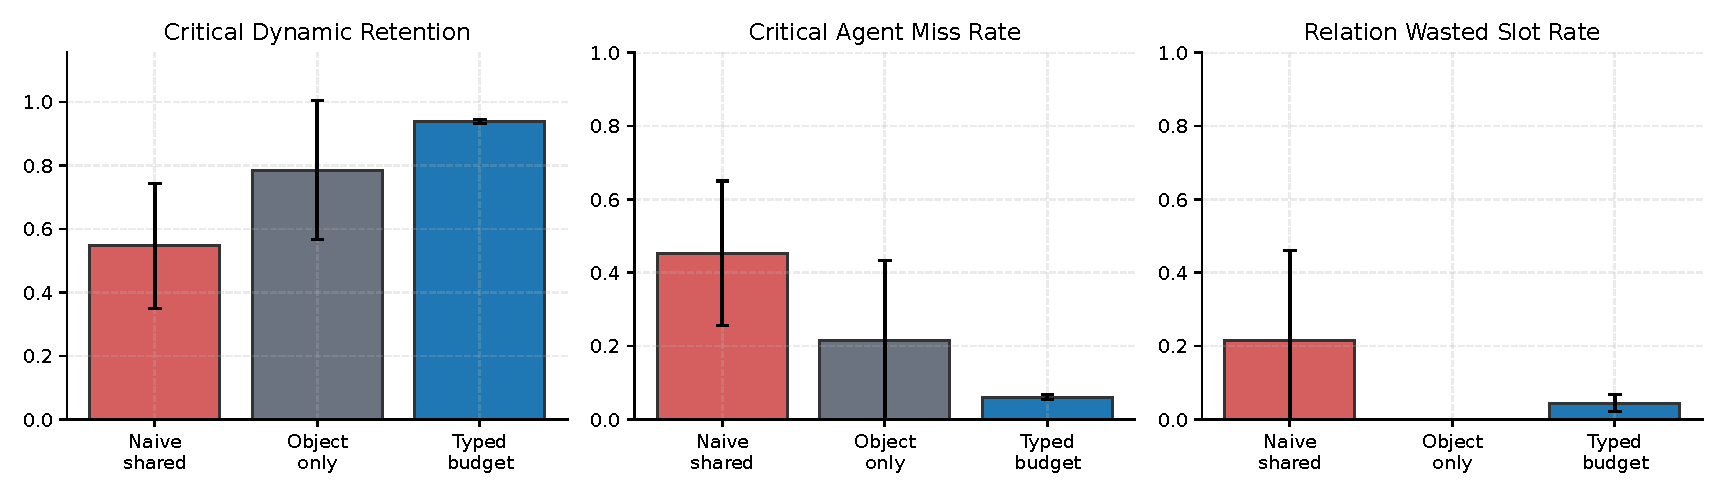
\includegraphics[width=0.92\textwidth]{fig_selection_diagnostics_bars}
\caption{Selection diagnostics. The typed-budget no-visibility condition has high Critical Dynamic Retention and low MissRate, while the naive shared-relation condition exhibits higher critical-agent misses and wasted relation slots.}
\label{fig:selection_bars}
\end{figure}

\begin{table}[t]
\centering
\caption{Aggregated selection diagnostic summary before the final 50k shared-relation closure. The naive shared-relation row uses the 20k diagnostic run; object-only and typed-budget rows use the 50k diagnostic run.}
\label{tab:selection_diag}
\begin{tabular}{lrrrrr}
\toprule
Condition & CDR $\uparrow$ & MissRate $\downarrow$ & WastedRel $\downarrow$ & ROI & MissRate--IntRec $\rho$ \\
\midrule
wm\_naive (20k) & 0.547 & 0.453 & 0.216 & 0.054 & -0.680 \\
wm\_object & 0.785 & 0.215 & N/A & 0.000 & -0.519 \\
wm\_decoupled\_no\_vis & \textbf{0.939} & \textbf{0.061} & \textbf{0.044} & 0.260 & -0.404 \\
\bottomrule
\end{tabular}
\end{table}

The 20k diagnostic already showed that shared top-$K$ can miss critical agents and waste relation slots, especially for seed 123. After the 50k shared-relation closure run completed, the same diagnostic exposed a sharper failure mode for the naive selector: two of three seeds retain fewer than 30\% of critical dynamic agents. Table~\ref{tab:selection_diag_50k_naive} reports the per-seed values. We therefore use the 50k shared-relation diagnostic as the main closure evidence and retain the 20k diagnostic as an earlier consistency check.

\begin{table}[t]
\centering
\caption{Selection diagnostic for the 50k naive shared object-relation condition. The aggregate CDR is $0.452 \pm 0.312$ and the aggregate MissRate is $0.548 \pm 0.312$.}
\label{tab:selection_diag_50k_naive}
\begin{tabular}{rrrrrrr}
\toprule
Seed & Samples & CDR $\uparrow$ & MissRate $\downarrow$ & WastedRel $\downarrow$ & ROI & IntRec@1m $\uparrow$ \\
\midrule
7 & 10000 & 0.298 & 0.702 & 0.377 & 0.082 & 0.007 \\
42 & 10000 & 0.812 & 0.188 & 0.201 & 0.389 & 0.765 \\
123 & 10000 & 0.247 & 0.753 & 0.274 & 0.160 & 0.001 \\
\bottomrule
\end{tabular}
\end{table}

\begin{figure}[t]
\centering
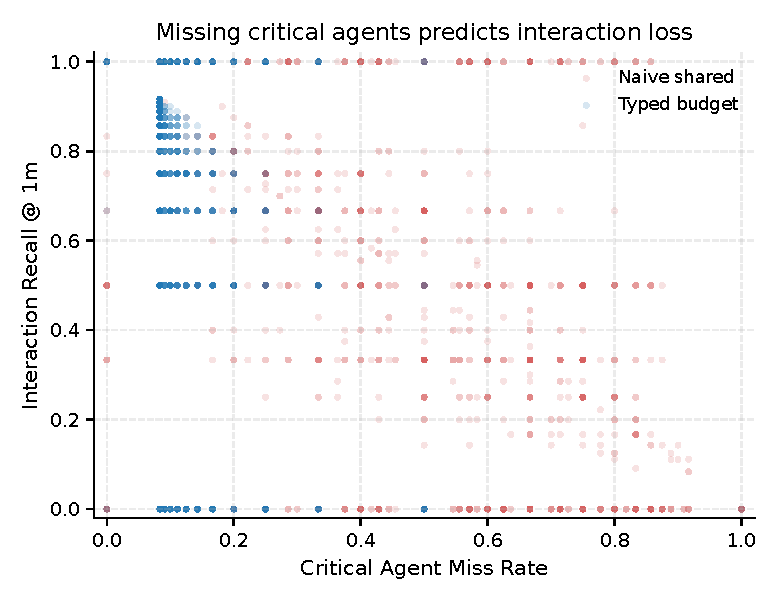
\includegraphics[width=0.72\textwidth]{fig_missrate_vs_interaction_recall}
\caption{Critical Agent Miss Rate versus Interaction Recall. The diagnostic is intended to connect selector behavior to interaction-sensitive representation quality rather than treating top-$K$ choices as an opaque implementation detail.}
\label{fig:missrate_intrec}
\end{figure}

\subsection{Latent Planning on nuPlan}
On nuPlan 50k, typed-budget no-visibility abstraction yields the strongest and most stable latent planning performance among the evaluated world-model conditions.

\begin{table}[t]
\centering
\caption{Stage 1 nuPlan 50k latent planning results.}
\label{tab:nuplan50k}
\begin{tabular}{lrrrr}
\toprule
Condition & Return $\uparrow$ & ImagColl $\downarrow$ & CollMean $\downarrow$ & Stability \\
\midrule
wm\_object & $1.723 \pm 17.886$ & $0.610 \pm 0.146$ & $0.614 \pm 0.113$ & 0.367 \\
wm\_decoupled & $-0.330 \pm 4.936$ & $\mathbf{0.007 \pm 0.012}$ & $0.277 \pm 0.111$ & 0.255 \\
wm\_decoupled\_no\_vis & $\mathbf{14.511 \pm 2.925}$ & $0.259 \pm 0.045$ & $\mathbf{0.277 \pm 0.033}$ & \textbf{0.222} \\
\bottomrule
\end{tabular}
\end{table}

\paragraph{Shared-relation 50k closure.}
We also ran the naive shared object-relation Stage-1 condition at the same 50k scale. The three seeds finished with returns $2.612$, $-6.713$, and $-2.807$, collision rates $0.000$, $0.245$, and $1.000$, and collision means $0.333$, $0.293$, and $0.725$, respectively. The aggregate is $-2.303 \pm 4.681$ return, $0.415 \pm 0.518$ imagined collision rate, and $0.450 \pm 0.239$ collision mean. This condition is better than the catastrophic Stage-0 representation failure would suggest for one seed, but it remains substantially weaker and less stable than typed-budget no-vis at 50k.

\subsection{Offline Planner-Like Alignment}
Latent return alone is not sufficient evidence for planning relevance, so we also evaluate offline teacher-action alignment on the nuPlan 50k validation split. This probe is not a closed-loop benchmark, but it asks whether the policy actions induced by the learned latent state align better with planner-derived action targets.

\begin{table}[t]
\centering
\caption{Offline planner-like sanity check on nuPlan 50k. Lower teacher action MSE and action $\Delta$L2 indicate better alignment with planner-derived action targets.}
\label{tab:offline_planner}
\resizebox{\textwidth}{!}{
\begin{tabular}{lrrrrrr}
\toprule
Condition & Teacher MSE $\downarrow$ & Action $\Delta$L2 $\downarrow$ & Return $\uparrow$ & CollRate $\downarrow$ & CollMean $\downarrow$ & Progress proxy $\uparrow$ \\
\midrule
wm\_object & $8.863 \pm 0.370$ & $3.553 \pm 0.118$ & $1.722 \pm 17.888$ & $0.610 \pm 0.146$ & $0.614 \pm 0.113$ & 2.995 \\
wm\_decoupled\_no\_vis & $\mathbf{6.628 \pm 0.110}$ & $\mathbf{2.115 \pm 0.083}$ & $\mathbf{14.512 \pm 2.925}$ & $\mathbf{0.259 \pm 0.045}$ & $\mathbf{0.277 \pm 0.033}$ & 1.082 \\
\bottomrule
\end{tabular}}
\end{table}

\subsection{Relation Semantics Matter: TTC/Risk Drives the Gain}
We probe relation semantics by ablating relation feature groups at evaluation time on trained \texttt{wm\_decoupled\_no\_vis} checkpoints. Removing TTC/risk nearly triples collision metrics, while removing lane/priority has little effect under the current tokenizer. This suggests that the useful relation information is concentrated in risk/TTC semantics rather than distributed uniformly across all relation features.

\begin{figure}[t]
\centering
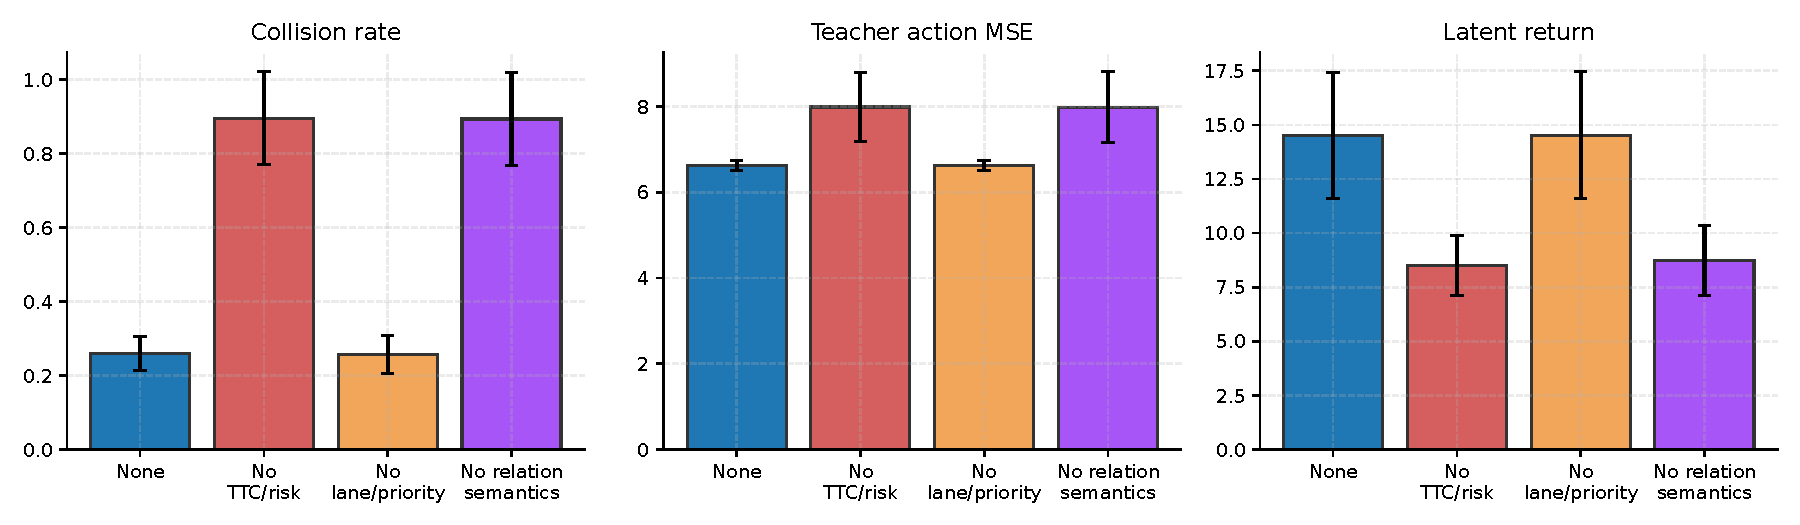
\includegraphics[width=0.92\textwidth]{fig_relation_semantics_ablation}
\caption{Relation semantic ablation on nuPlan 50k. Removing TTC/risk strongly degrades collision and teacher-action metrics, while removing lane/priority is close to neutral.}
\label{fig:relation_ablation}
\end{figure}

\begin{table}[t]
\centering
\caption{Relation feature-group ablation on nuPlan 50k.}
\label{tab:relation_ablation}
\resizebox{\textwidth}{!}{
\begin{tabular}{lrrrrr}
\toprule
Ablation & Teacher MSE $\downarrow$ & Action $\Delta$L2 $\downarrow$ & Return $\uparrow$ & CollRate $\downarrow$ & CollMean $\downarrow$ \\
\midrule
none & $\mathbf{6.628 \pm 0.110}$ & $2.115 \pm 0.083$ & $14.510 \pm 2.921$ & $0.260 \pm 0.045$ & $0.277 \pm 0.033$ \\
no\_ttc\_risk & $7.992 \pm 0.805$ & $3.154 \pm 0.335$ & $8.498 \pm 1.397$ & $0.895 \pm 0.126$ & $0.891 \pm 0.126$ \\
no\_lane\_priority & $\mathbf{6.627 \pm 0.111}$ & $\mathbf{2.113 \pm 0.081}$ & $\mathbf{14.526 \pm 2.931}$ & $\mathbf{0.257 \pm 0.052}$ & $\mathbf{0.274 \pm 0.040}$ \\
no\_relation\_semantics & $7.989 \pm 0.827$ & $3.151 \pm 0.351$ & $8.724 \pm 1.629$ & $0.894 \pm 0.126$ & $0.888 \pm 0.127$ \\
\bottomrule
\end{tabular}}
\end{table}

\subsection{External-Style Imitation Anchor}
We include a low-cost BC / planner-target imitation baseline on the same nuPlan 50k protocol. It is not intended to beat the world-model method; its role is to ensure that the paper is not purely comparing internal variants. The BC baseline reaches return $0.433 \pm 4.230$ and teacher-action MSE $8.824 \pm 0.113$, below \texttt{wm\_decoupled\_no\_vis} in latent return and teacher-action alignment.

\subsection{Budget Sensitivity}
We evaluate a more relation-heavy $(\kdyn,\krel)=(10,6)$ split against the main $(12,4)$ split. The 10/6 budget is runnable but substantially weaker: DynRoll increases from $1.876 \pm 0.227$ to $8.761 \pm 1.067$, Rare ADE increases from $0.520 \pm 0.049$ to $1.574 \pm 0.485$, and IntRec@1m drops from $0.979 \pm 0.008$ to $0.884 \pm 0.043$. This supports using 12/4 as the default typed budget rather than a relation-heavy allocation.

\begin{figure}[t]
\centering
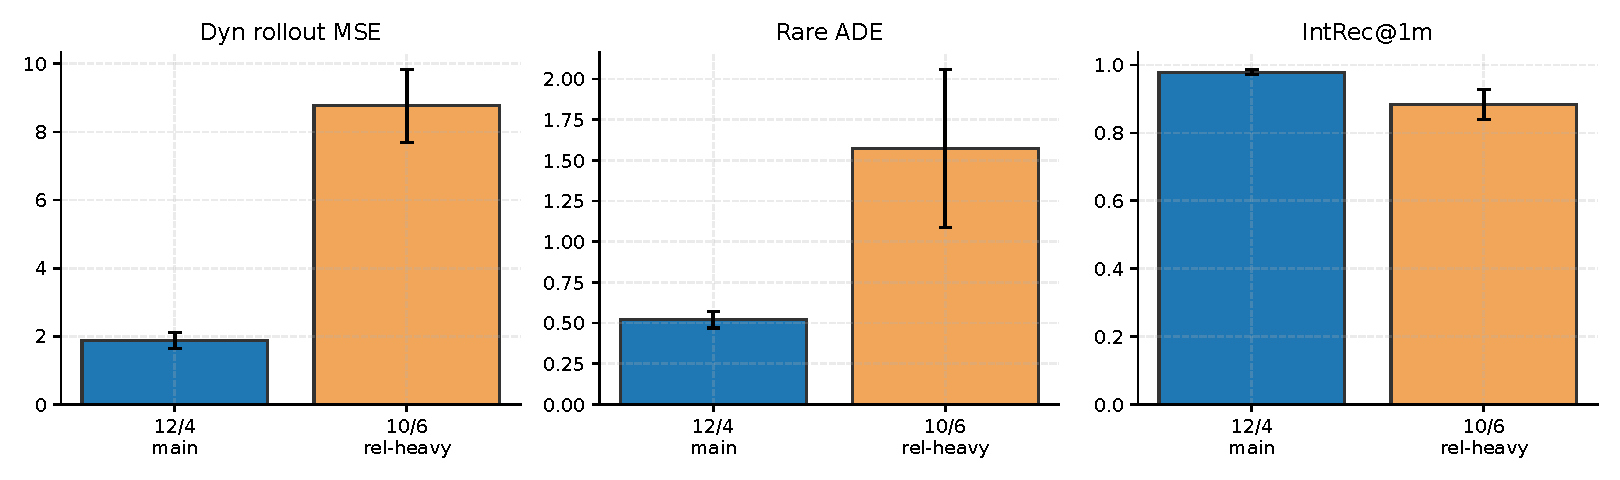
\includegraphics[width=0.92\textwidth]{fig_budget_sensitivity_12_4_vs_10_6}
\caption{Budget sensitivity. A relation-heavy 10/6 split underperforms the main 12/4 split on nuScenes Stage 0, showing that reserving too many relation slots can again harm dynamic-agent sufficiency.}
\label{fig:budget}
\end{figure}

\section{Discussion}
\paragraph{Type competition, not bad relations.}
The central result is not that relation tokens are harmful. Relation tokens can be useful, especially TTC/risk features. The problem is that relation tokens need to be grounded in retained dynamic state. A shared top-$K$ selector can spend capacity on relation tokens while missing the objects that make those relations meaningful. Budget-aware type abstraction prevents this by reserving capacity for state-bearing agents and decision-dense relations separately.

\paragraph{Why not learn the budget?}
A natural extension is to learn $\kdyn$ and $\krel$ dynamically. We leave this for future work. The point of the present paper is to establish the failure mode and show that a simple structural prior fixes it under a strict fixed total budget. Adding learned budget allocation would introduce a second layer of optimization and make the mechanism harder to isolate.

\paragraph{Why relation density alone is insufficient.}
We originally hypothesized that relation density would directly predict relation over-allocation. The current diagnostics do not strongly support that chain. This negative result is useful: type competition is not merely a function of how many relation tokens exist. It depends on whether relation selection displaces critical dynamic state and whether selected relations remain grounded.

\section{Limitations}
First, current relation tokens are largely ego-object relations, and endpoint ids are recovered for diagnostics by nearest dynamic-token matching. Future tokenizers should store explicit relation endpoints. Second, the main typed budget uses a fixed 12/4 split. We include sensitivity evidence, but do not yet learn budgets dynamically. Third, latent planning metrics are not a substitute for full high-fidelity closed-loop evaluation. Finally, relation utility varies across datasets and planning regimes; this paper frames that variation as part of the phenomenon rather than hiding it.

\section{Reproducibility and Artifact Map}
Key implementation files are \texttt{src/doorrl/models/doorrl\_variant.py}, \texttt{src/doorrl/models/abstraction.py}, \texttt{src/doorrl/training/losses.py}, \texttt{src/doorrl/evaluation/table3\_metrics.py}, \texttt{src/doorrl/evaluation/stage1\_metrics.py}, and \texttt{scripts/selection\_diagnostic.py}. Key experiment outputs include \texttt{experiments/table3\_fair\_fix2\_aggregate.json}, \texttt{experiments/nuplan\_stage1\_50k/summary.md}, \texttt{experiments/nuplan\_stage1\_shared\_relation\_50k/seed*/wm\_naive/stage1\_metrics.json}, \texttt{experiments/selection\_diagnostic\_nuplan50k/summary.md}, \texttt{experiments/selection\_diagnostic\_shared\_relation\_20k/summary.md}, \texttt{experiments/selection\_diagnostic\_shared\_relation\_50k/}, \texttt{experiments/nuplan\_relation\_feature\_ablation\_50k/summary.md}, \texttt{experiments/nuplan\_bc\_baseline\_50k/summary.md}, and \texttt{experiments/stage0\_budget\_10\_6\_nuscenes/summary.md}.

\section*{Acknowledgments}
This is an internal manuscript draft. Replace this paragraph with final acknowledgments before submission.

\bibliographystyle{plainnat}
\bibliography{doorrl_refs}

\end{document}
